%%%%%%%%%%%%%%%%%%%%%%%%%%%%%%%%%%%%%%%%%%%%%%%%%%%%%%%%%%%%%%%%%%%%%%%%%%%%%%%%
%2345678901234567890123456789012345678901234567890123456789012345678901234567890
%        1         2         3         4         5         6         7         8

\documentclass[letterpaper, 10 pt, conference]{ieeeconf}  % Comment this line out
                                                          % if you need a4paper
%\documentclass[a4paper, 10pt, conference]{ieeeconf}      % Use this line for a4
                                                          % paper

\IEEEoverridecommandlockouts                              % This command is only
                                                          % needed if you want to
                                                          % use the \thanks command
\overrideIEEEmargins
% See the \addtolength command later in the file to balance the column lengths
% on the last page of the document

\usepackage{graphicx,float}
\usepackage{caption}
\usepackage{subcaption}
\usepackage{subfig}
\usepackage{mathrsfs}
\usepackage{amsmath,amssymb}
\usepackage{mathtools}
\usepackage{icra_2014_initial}
\usepackage{url}
\usepackage{comment}


\newtheorem{mydefinition}{\bfseries Definition}%[section]
\newtheorem{mynote}{\bfseries Note}%[section]
\newtheorem{myproposition}{\bfseries Proposition}%[section]
\newtheorem{myexample}{\bfseries Example}%[section]
\newtheorem{myassumption}{\bfseries Assumption}%[section]
\newtheorem{mytheorem}{\bfseries Theorem}
\newtheorem{mymaintheorem}{\bfseries Main Theorem}
\newtheorem{mycorollary}{\bfseries Corollary}%[section]
\newtheorem{mylemma}{\bfseries Lemma}%[section]
\newtheorem{myproperty}{\bfseries Property}
\newtheorem{myremark}{\bfseries Remark}
\newtheorem{mynotation}{\bfseries Notation}

\title{\LARGE \bf
Planar Multi-Contact Bipedal Walking Using Hybrid Zero Dynamics and Quadratic Programs
}
\author{\authorone, \authortwo, and \authorthree% <-this % stops a space
  \thanks{\authorone, \text{\authortwo} and \text{\authorthree} are with the Department of Mechanical Engineering, Texas A\&M University, College Station, TX 77843, e-mail:
    {\tt\small \{jordanlack,mjpowell,aames\}@tamu.edu}}%
    \thanks{This research is supported by NASA grant NNX11AN06H, NSF grants CNS-0953823 and CNS-1136104, and NHARP award 00512-0184-2009.}% <-this % stops a space
}

\begin{document}

\maketitle
\thispagestyle{empty}
\pagestyle{empty}

\begin{abstract}
This paper presents a method for achieving planar multi-phase, multi-contact robotic walking using a human inspired
control and optimization. The walking presented contains phases with differing degrees of actuation including
over actuated double support, fully actuated single support, and under actuated single support via
heel lift. An optimization methodology for generating walking gaits will be presented utilizing partial hybrid zero dynamics.  It will be shown that this method yields periodic, multi-contact locomotion. In addition, a control law utilizing online optimization via 
a quadratic program will be presented, resulting in improved controller 
capabilities and performance. Simulation results for both standard Input-Output Linearization as well as the quadratic program will be presented.
\end{abstract}

\input{sections/sec_introduction}
\section{Hybrid Control System Model}
\label{sec:hybridsystems}

This section develops the mathematical model for multi-contact locomotion for a bipedal robot with feet.  In particular, the changing of contact points over a walking gait, e.g., lifting and striking of the heel and toe, necessitates a model of the bipedal robot that includes continuous and discrete dynamics.  For this paper the goal will be to construct a walking gait with three discrete domains (see Fig. \ref{fig:DomainGraph}) consisting of a phases of single \emph{and} double support.

\begin{figure}[t]
\centering
%\hspace{-12mm}
\includegraphics[width=0.35\textwidth]{figures/DomainGraph.pdf}
\caption{Directed graph associated with 3 domain walking. The red leg is the stance leg and the black leg is the non-stance leg.}
\label{fig:DomainGraph}
\end{figure}

\newsec{Hybrid System Model.}
The formal model of a bipedal robot with a multi-contact multi-domain walking gait follows the general development given in \cite{SPSA:IFAC:11}.  In particular, we consider a {\it hybrid control system model} given by a tuple:
 \begin{align}
 \label{eqn:HC}
  \HC = (\Gamma, \domain, \admissiblecontrol, \guard, \resetmap, \controlsystem),
 \end{align}
 where $\Gamma = (V,E)$ is a directed graph with vertices and edges,
  $D$ a set of domains, $U$ a set of admissible controls, $\Delta$ a set of reset maps, and $FG$ a control system. For a generalized definition of each element we refer the reader to \cite{SPSA:IFAC:11}.
The remainder of this section will be devoted to defining the specific elements of this hybrid system in the context of the multi-domain walking gait of interest. 

\newsec{Graph Structure.}  For the multi-contact walking gait of interest, the graph $\Gamma$ of the hybrid system $\HC$ is pictured in Fig. \ref{fig:DomainGraph}.   In particular, the discrete structure of the walking gait implies that $\Gamma$ is a directed cycle, with vertices and edges given by:
\begin{align}
 \VertexSet &= \{ \oa, \fa , \ua \}\\
 \EdgeSet   &= \{ \ts = (\ds \to \fa),\hl =(\fa \to \ua), \hs = (\ua \to \ds) \}.\nonumber
\end{align}
where in this case, we have labeled the vertices (also referred to as domains) by the type of actuation each of these domains display (as will be discussed later), i.e., the vertices $\oa$, $\fa$ and $\ua$ correspond to over, full and under actuation, respectively. 

\begin{figure}
\begin{subfigure}{0mm}
\includegraphics[width=40mm]{figures/RobotCoords.pdf}
\end{subfigure}
\hbox{\hspace{40mm}
\begin{subfigure}{0mm}
\includegraphics[width=50mm]{figures/RobotConfig.pdf}
\end{subfigure}}
\caption{Coordinates of 9 degree of freedom footed biped model (left) and layout of physical parameters (right).}
\label{fig:robotCoords}
\end{figure}


\newsec{Coordinates, Constraints and Actuation Types.}
We will now introduce basic terminology related to coordinates, constraints and actuation types that will be necessary to define the hybrid control system \eqref{eqn:HC} modeling a planar bipedal robot exhibiting a multi-domain walking gait. In particular, due to the multi-domain structure of the hybrid system model, this involves considering the generalized coordinates of the robot $Q = \mathbb{R}^{2} \times SO(2) \times Q_{r}$ where $Q_{r}$ is characterized by the relative joint angles(see Fig \ref{fig:robotCoords}). Specifically, $q = \{p_{x},p_{z},\varphi_{0},q_{r}\}$ where $q_{r} = \{q_{sa},q_{sk},q_{sh},q_{nsh},q_{nsk},q_{nsa}\}$ and $\{p_{x},p_{z},\varphi_{0}\}$ reference the body fixed frame $R_{b}$ with respect to a fixed inertial frame $R_{0}$ shown in Fig. \ref{fig:robotCoords}.
% : $Q = \Reals^2 \times SO(2) \times Q_r$, where $Q_r$ is the (relative) configuration space of the robot characterized by the relative angles of the system.  We assume that a subset of $Q_r$ are chosen so that there is a well-defined coordinate system, i.e., so that $Q_r$ is embeddable in $\Reals^{n_r}$, $Q_r \subset \Reals^{n_r}$, with coordinates expressed as $q_r \in Q_r$.  The generalized coordinate space $Q \subset \Reals^{n}$,  can be expressed in coordinates as $q = (p^T,\varphi_{0},q_r)^T$, where $p = (p^x,p^y)^T$ is a point and $\varphi_{0} \in SO(2)$ is an angle expressing the position and orientation of a reference frame, $R_b$, attached to the body of the robot relative to a world frame $R_0$.

% \gap

% \begin{myexample}
% For the simulation results presented in this paper (see Sec. \ref{sec:simresults}), the bipedal robot AMBER 2 will be considered; this robot can be seen in Fig. \ref{fig:robots}.  For this robot, the configuration space is given by $\indexbyrobot{\q} = \{ \qsa, \qsk, \qsh, \qnsh, \qnsk, \qnsa\}$, with the specific joint angles shown in Fig. \ref{fig:robotCoords}. 
% \end{myexample}

% \gap

{\it Contact Conditions:}  For each vertex of the graph $\Gamma$, there are associated contact points interacting with the physical world that dictate multi-contact conditions in the robot \cite{AVB:HSCC:11}. 
 This is represented by a set of contact points $\ContactSet = \{ sh, st, nsh, nst\}$, where $sh$ is the stance-heel, $st$ is the stance-toe, $nsh$ is the non-stance heel and $nst$ is the non-stance toe. With this, we consider two types of constraints: \emph{unilateral}, denoted $h_{v}$, and \emph{holonomic}, denoted $\eta_{v}$. Unilateral constraints dictate the set of admissible configurations, while holonomic constraints are used to encode which points are in contact with the walking surface.
 % indicating which points on the robot can, or are, interacting with the world.  Since we are considering a planar robot locomoting, we need only consider the contact points associated with the feet, i.e., $sh$ is the stance-heel, $st$ is the stance-toe, $nsh$ is the non-stance heel and $nst$ is the non-stance toe.  Associated with the indexing set of contact points are two types of constraints: {\it unilateral} and {\it holonomic}.   Unilateral constraints, denoted by $h_v$ for $v \in V$, are a vector-valued function that dictates the admissible configurations of the system on each domain by codifying which contact points are not on the ground, and therefore must stay above the ground for the current contact configuration to hold true.  Conversely, holonomic constraints, denoted by $\eta_v$ for $v\in V$, is a vector-valued function encoding which contact points are in contact with the ground and, therefore, must be held constant. 

\begin{myexample}
To provide a specific example, for the domain structure considered in this paper (see Fig. \ref{fig:DomainGraph}) there are the following constraints for each domain:
 \begin{itemize}
 \item For $v = \fa \in V$, $h_{\fa}(q)$ is the vertical reaction force at the stance heel, and $\eta_{\fa}(q)$ consists of the $x$, $z$ position of the stance toe together with the $z$ position of the stance heel.
\item For $v = \ua \in V$, $h_{\ua}(q)$ consists of the $z$ position of the non-stance heel, while $\eta_{\ua}(q)$ consists of the $x$, $z$ position of the stance toe.
\item For $v = \oa \in V$, $h_{\oa}(q)$ consists of the $z$ position of the stance toe, while $\eta_{\oa}(q)$ consists of the $x$, $z$ position the stance heel and the $z$ position of the stance toe.
 \end{itemize}
\end{myexample}

\gap

{\it Actuation Type:}  With notions of coordinates and constraints in hand, we wish to make explicit what is meant by full, over and under actuation. Let $m_r$ denote the number of actuators of the robot, $n = 9$ the number of unconstrained degrees of freedom of the robot, and $n_{c_v}$ denote the number of holonomic constraints in a given domain $v \in V$.  We say that a domain, $v \in V$, is
\begin{itemize}
 \item {\it Fully-actuated} if  $m_r = n - n_{c_v}$,
 \item {\it Under-actuated} if $m_r < n - n_{c_v}$,
 \item {\it Over-actuated} if  $m_r > n - n_{c_v}$. 
\end{itemize}
Similarly, we define the $V_{fa}$ to be the set of full-actuated domains, $V_{ua}$ to be the set of under-actuated domains, and $V_{oa}$ to be the set of over-actuated domains. 

\gap

\begin{myexample}
AMBER 2 has six actuators, thus $m_{r} = 6$. For $\oa \in V$, $n_{c_{\oa}} = 4$ thus $n - n_{c_{\oa}} = 9 - 4 = 5 < 6$ and the robot is over-actuated in $\oa$. For $\fa$, $n_{c_{\fa}} =3$ thus $n - n_{c_{\fa}} = 9 - 3 = 6$ and therefore the robot is said to be fully-actuated in $\fa$. For $\ua$, $n_{c_{\ua}}=2$ thus $n - n_{c_{\ua}} = 9 - 2 = 7>6$ and therefore the robot is under-actuated in $ua$. Note that it is useful to refer to this example when reading Section \ref{sec:control}.
\end{myexample}


\newsec{Continuous Dynamics.}
 We now have the necessary framework in which to construct the control system 
 \begin{align}
 \label{eqn:fgdyn}
 \xdot = \indexbyvertex{f}(\x) + \indexbyvertex{g}(\x) \control, \qquad v \in V
 \end{align}
 for each domain of the hybrid system $\HC$ given in \eqref{eqn:HC} where $x = (q,\dot{q})$.  In particular, the dynamics on each domain will be obtained from general ``unpinned'' dynamics through the use of holonomic constraints.

We begin by considering the unconstrained dynamics of the robot, i.e., the ``unpinned'' dynamics of the robot obtained by assuming no contact with the environment. Holonomic constraints are then used to enforce contact conditions. For a detailed derivation of the constrained dynamics we refer the reader to \cite{GCAS10}. The resulting constrained dynamical system is described by,
% \begin{align}
%  \nonumber
%  \Lagrangian(\q,\dq) = \frac{1}{2} \dq^T M(q) \dq  - \PotentialEnergy(\q), 
% \end{align}
% with $\GeneralizedInertia$ the generalized inertia matrix.  The Euler-Lagrange equations yield the equations of motion, which for robotic systems \cite{MLS94} are of the form:
% \begin{align}
%  \label{eq_eulerlagrange}
%  \GeneralizedInertia\ddq + \CoriolisGravity = \TorqueDistribution \control,
% \end{align}
% where $\CoriolisGravity = \Coriolis + \Gravity$ contains the Coriolis and gravity effects, $\TorqueDistribution$ is the torque distribution matrix, and $\control$ is the vector of actuator torques.
% Recall that for a domain $\vertex \in \VertexSet$, the holonomic constraints that are imposed on that domain are given by $\indexbyvertex{\holonomic}(\q)$.  Differentiating the holonomic constraints yields the constraint:
% \begin{align}
% \label{eqn:JT}
%  \indexbyvertex{\Jacobian}(\q) \dq = 0,
% \end{align}
% where $\indexbyvertex{\Jacobian}(\q) = \text{RowBasis} (\frac{\partial \indexbyvertex{\holonomic}(\q)}{\partial \q})$ is a basis for the row space of the Jacobian (this removes any redundant constraints so that $\indexbyvertex{\Jacobian}$ has full row rank). The constraint \eqref{eqn:JT} yields the \textit{constrained dynamics} on each domain $v \in V$:
\begin{align}
 \GeneralizedInertia\ddq + C(q,\dot{q})\dot{q} + G(q) = \TorqueDistribution \control + \indexbyvertex{\Jacobian}(q)^T \indexbyvertex{\ContactWrench}
 \label{eq_eulerlagrangeconstrained}
\end{align}
which enforces the holonomic constraint; here $\GeneralizedInertia$, $C(q,\dot{q})$ and $G(q)$ are the inertia matrix, coriolis matrix, and gravity vector and $\indexbyvertex{\ContactWrench}$ is the \textit{wrench} containing forces and moments expressed in the reference frame body frame \cite{GCAS10}. The constrained dynamics along with the holonomic constraints allows for the contact wrench to be solved for in terms of the state variables and joint torques(see \cite{GCAS10}).
% To determine the wrench $\indexbyvertex{\ContactWrench}$, we differentiate the kinematic constraint:
% \begin{align}
% \label{eqn:JJdotequaiton}
%  \indexbyvertex{\Jacobian}(q) \ddq + \dot{J}_v(q) \dq = 0,
% \end{align}
% and combine this equation with \eqref{eq_eulerlagrangeconstrained} to obtain an expression for $\indexbyvertex{\ContactWrench} (\q,\dq,\control)$ which is affine in $\control$. Therefore, by defining $\x = (\q^T, \dq^T)^T$, \eqref{eq_eulerlagrangeconstrained} and \eqref{eqn:JJdotequaiton} yields the affine control system of the form \eqref{eqn:fgdyn}. 

\newsec{Discrete Dynamics.} We now construct the continuous domains, $D$, guards, $S$, and reset maps $\Delta$, for a hybrid system \eqref{eqn:HC} using the unilateral and holonomic constraints.

Given a vertex $\vertex \in \VertexSet$, the continuous domain is the set of admissible configurations of the system factoring in both friction and a unilateral constraint. Specifically, from the wrench $\indexbyvertex{\ContactWrench} (\q,\dq,\control)$, one can ensure that the foot does not slip by considering inequalities on the friction which can be stated in the form: $\indexbyvertex{\frictioncoefficient}(q)^T \indexbyvertex{\ContactWrench}(\q,\dq,\control) \geq 0$, with $\indexbyvertex{\frictioncoefficient}$ a matrix of friction parameters (see \cite{SPSA:IFAC:11} for more details). These are coupled with the unilateral constraint on this domain, $\indexbyvertex{\unilateral}(q)$, to yield the set of admissible configurations:
\begin{align}
\indexbyvertex{\ConstraintMatrix}(\q,\dq,\control) &= \left[
  \begin{array}{c}
    \indexbyvertex{\frictioncoefficient}(q)^T \indexbyvertex{\ContactWrench}(\q,\dq,\control) \\
    \indexbyvertex{\unilateral}(q)
  \end{array}
  \right] \geq 0.
\end{align}
The continuous domain is thus given by:
\begin{align}
 \indexbyvertex{\domain} = \{ (\q,\dq,\control) \in TQ \times \Reals^{\indexbyvertex{\dimensionu}} : \indexbyvertex{\ConstraintMatrix}(\q,\dq,\control) \geq 0 \}.
\end{align}
The guard is just the boundary of this domain with the additional assumption that the set of admissible configurations is decreasing, i.e. the vector field is pointed outside of the domain, or for an edge $\edge =(\vertex \to \vertex') \in \EdgeSet$,
\begin{align}
 \indexbyedge{\guard} = \{ (\q,\dq,\control) \in TQ \times \Reals^{\indexbyvertex{\dimensionu}} : h_{v} = 0 \hspace{1mm} \\
  \nonumber \text{and} \hspace{1mm} \dot{h}_{v} < 0\}.
\end{align}
%\begin{align}
% \indexbyedge{\guard} = \{ (\q,\dq,\control) \in TQ \times \Reals^{\indexbyvertex{\dimensionu}} : \indexbyvertex{\ConstraintMatrix}(\q,\dq,\control) = 0 \hspace{1mm} \\
%  \nonumber \text{and} \hspace{1mm} \indexbyvertex{\dot \ConstraintMatrix}(\q,\dq,\control) < 0\}.
%\end{align}
The impact equations are given by considering the holonomic constraints enforced on the subsequent domain.  In particular, the post-impact velocity $\dq^+$ is given in terms of the pre-impact velocity $\dq^-$. With this, the reset map\footnote{Note that as a result of considering ``stance'' and ``non-stance'' legs, the labeling on the legs must be switching during one of the transitions; in this paper, these switching occurs at heel strike.  This is a common ``trick'' in robotic walking used to reduce the number of discrete domains.} is given by,
% \begin{align}
%  \dq^+ & = \indexbyedge{P}(\q, \dq^-)  \\
%    & = (I - \GeneralizedInertia^{-1} \Jacobian_{\vertex'}^T (\Jacobian_{\vertex'} \GeneralizedInertia^{-1} \Jacobian_{\vertex'}^T)^{-1} \Jacobian_{\vertex'}) \dq^-
% \end{align}
\begin{align}
 \indexbyedge{\resetmap}(\q,\dq) = \left[
    \begin{array}{c}
      \q \\
      \indexbyedge{P}(\q,\dq)
    \end{array}
    \right]
\end{align}
where $P_{e}$ is computed from the impact equations assuming perfectly plastic impacts(see \cite{WGCCM07}). The end result is that the hybrid model for the biped of a 2D bipedal robot is now completely defined.


\input{sections/sec_control_ames}
\input{sections/sec_optimization}
\input{sections/QuadraticProgram}
\input{sections/sec_simresults}
\section{Conclusion}

The objective of this paper has been to present a novel method with which to design multi-domain walking gaits. It began with the introduction of multi-domain hybrid systems followed by the introduction of the floating base model. The principle contribution lies, however, in the multi-domain human inspired optimization. Using the human inspired optimization, walking gaits can be designed and shaped by altering constraints. The human-like walking presented here was achieved using I/O Linearization, but with the use of a QP a single control law to be used for domains with differing degrees of actuation. The methods described here have been recently realized on AMBER 2 to achieve robust, multi-domain locomotion \cite{url:AMBER2_MultiContact}.

\bibliographystyle{abbrv}
\bibliography{bibdata}

\end{document}
